\documentclass{beamer}
\usetheme{metropolis}
\usepackage{tikz}
\usepackage{minted}

\usepackage{algorithm}
\usepackage{algorithmic}

\makeatletter %
\newcommand{\JuMP}
{
J%
{%
  \sbox \z@ T%
  \vbox to\ht \z@ {%
    \hbox {%
      \check@mathfonts%
      \math@fontsfalse%
      \selectfont%
      u%
    }%
    \vss%
  }%
}%
MP
}
\makeatother%

\title{Automatic reformulation using constraint bridges}
\author{Beno\^it Legat (UCL)}
\institute{Universit\'e catholique de Louvain (UCL)}

\begin{document}
\maketitle
\begin{frame}[fragile]
  \frametitle{Motivation}
  Consider interval constraints:
\begin{minted}{Julia}
@constraint(m, 0 <= 2x + 3y <= 1)
\end{minted}
  and second order cone (SOC) constraints: %
\begin{minted}{Julia}
@constraint(m, x'*x <= t^2)
@constraint(m, [t; x] in MOI.SecondOrderCone(length(x)+1))
\end{minted}
  \begin{itemize}
    \item Solver A: supports interval constraints and quadratic constraints
    \item Solver B: does \alert{not} supports interval constraints and support SOC constraints.
  \end{itemize}
  What should \JuMP{} do ?
\end{frame}

\begin{frame}
  \frametitle{Solution 1}
  Disallow using interval constraints
  \begin{block}{Issues}
    \begin{itemize}
      \item Solver A benefits from knowing more stucture
      \item Does not work for SOC constraints
    \end{itemize}
  \end{block}
\end{frame}

\begin{frame}
  \frametitle{Solution 2}
  The user needs to enter the form supported by the solver
  \begin{block}{Issues}
    \begin{itemize}
      \item The user needs to read solvers docs
      \item Some transformations are not easy, let alone transforming duals
      \item Cannot write solver independent code
    \end{itemize}
  \end{block}
  Similar to MathProgBase LinearQuadraticModel/ConicModel/NLPModel with \JuMP{} v0.18 traits.
\end{frame}

\begin{frame}
  \frametitle{Solution 3}
  Write transformations in \JuMP{}
  \begin{block}{Issues}
    \begin{itemize}
      \item Bloat \JuMP{} code (need to transform duals!)
      \item Unfair: specific transformations are included and some are not
      \item Not extensible/distributed
    \end{itemize}
  \end{block}
  Similar to handling of PSD constraints in \JuMP{} v0.18.
\end{frame}

\begin{frame}
  \frametitle{Solution 4: Constraint Bridges}
  \begin{itemize}
      \item Transparent
      \item Lightweight
      \item Complete
      \item Extensible
  \end{itemize}
\end{frame}

\begin{frame}
  \frametitle{Transparent}
  Transparently bridge constraints by adding an MOI layer
  \begin{center}
    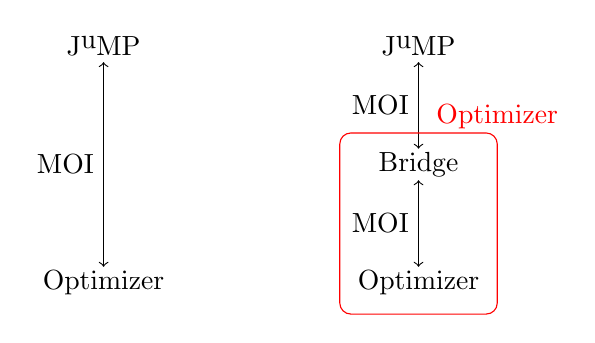
\begin{tikzpicture}
      \node at   (-2, 0) {\JuMP{}};
      \draw[<->] (-2, -0.2) to node[left] {MOI}
                 (-2, -2.8);
      \node at   (-2, -3) {Optimizer};
      \node at   ( 2, 0) {\JuMP{}};
      \draw[<->] ( 2, -0.2) to node[left] {MOI}
                 ( 2, -1.3);
      \node at   ( 2, -1.5) {Bridge};
      \draw[<->] ( 2, -1.7) to node[left] {MOI}
                 ( 2, -2.8);
      \node at   ( 2, -3) {Optimizer};
      \draw [rounded corners, color=red] (1, -3.4) rectangle (3, -1.1);
      \node[color=red] at (3, -0.9) {Optimizer};
    \end{tikzpicture}
  \end{center}
\end{frame}

\begin{frame}
  \frametitle{Lightweight}
  Transformed \emph{on the fly}, \alert{no copy} needed.

  MathProgBase bridges: model-wise $\to$ need full \alert{copy}.

  \begin{center}
    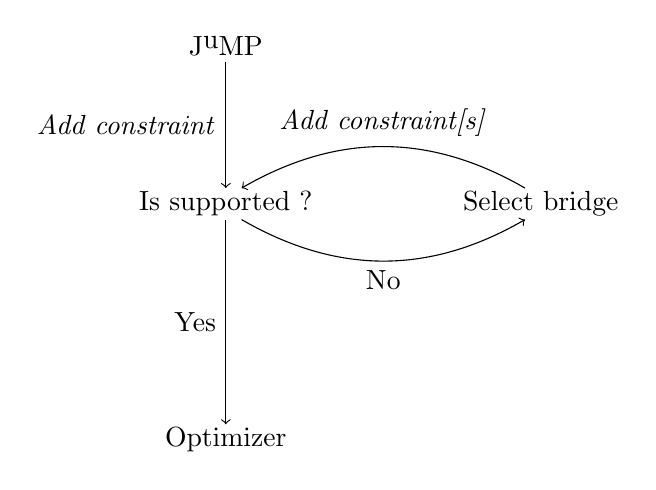
\begin{tikzpicture}
      \node at   (0, 2) {\JuMP{}};
      \draw[->]  (0, 1.8) to node[left] {\emph{Add constraint}}
                 (0, 0.2);
      \node at   (0, 0) {Is supported ?};
      \draw[->]  (0, -0.2) to node[left] {\alert{Yes}}
                 (0, -2.8);
      \draw[->, bend right]  (0.2, -0.2) to node[below] {\alert{No}}
                 (3.8, -0.2);
      \node at   (4, 0) {Select bridge};
      \draw[->, bend right]  (3.8, 0.2) to node[above] {\emph{Add constraint[s]}}
                 (0.2, 0.2);
      \node at   (0, -3) {Optimizer};
    \end{tikzpicture}
  \end{center}

\end{frame}

\begin{frame}
  \frametitle{Complete}
  If the underlying optimizer fully implements MOI,
  the bridged optimizer should too!

  Bridges keep indices of created constraints and variables
  and implements
  \begin{itemize}
      \item transforming constraint primal and constraint dual,
      \item deleting the constraint,
      \item modifying the constraint,
      \item remove indices of created constraints and variables from
        \texttt{MOI.ListOfVariableIndices}, ...
  \end{itemize}
  Keep original constraint for gett \texttt{MOI.ConstraintFunction},
  \texttt{MOI.ConstraintSet}, ...
\end{frame}

\begin{frame}%
  \frametitle{Transforming constraint duals}
  \begin{block}{Linear bridge from \texttt{*}-in-$S_1$ to \texttt{*}-in-$S_2$.}
  Suppose
  \[ x \in S_1 \Leftrightarrow Ax \in S_2 \qquad AS_1 = S_2 \]
  Hence
  \[ A^* y \in S_1^* \Leftrightarrow y \in S_2^* \qquad S_1^* = A^* S_2^* \]

  In Lagrangian:
  \[ \langle Ax, y \rangle_2 = \langle x, A^* y \rangle_1 \]
  \end{block}
\end{frame}

\begin{frame}
  \frametitle{Extensible}
  \alert{Custom} bridges can be added.
  How do we select bridges ?

  \begin{block}{Example}
    Root-Det constraint: $t \le \sqrt[d]{\det(X)}$, $X \in \mathbb{R}^{d \times d}$.

    Geometric-Mean constraint: $x \ge 0, t \le \sqrt[n]{x_1 x_2 \cdots x_n}$
    \begin{itemize}
      \item Bridge 1: Root-Det $\to$ PSD to get eigenvalues and GeoMean with eigenvalues.
      \item Bridge 2: GeoMean $\to$ Rotated SOC.
      \item Bridge 3: GeoMean $\to$ Power Cone (see Ulf's talk on Wednesday).
    \end{itemize}
  \end{block}
  \vspace{-1em}
  Which one to choose ?

  Select bridge that minimize the \alert{number} of bridges needed ?

  What do to for Bridge 2 and 3 ? Add \alert{cost} to bridges ?
\end{frame}

\begin{frame}
  \frametitle{What is our graph ? Directed Hypergraph}
  \begin{block}{Nodes}
    Each $F$-in-$S$ constraint types.
    Need to go beyond MOI's $F$ and $S$.
    It can by \alert{anything} for \alert{extensibility}.

    \alert{Infinitely} many nodes, we need to be \alert{lazy}!
  \end{block}
  \begin{block}{Edge}
    Each bridge $b$ defined possible \alert{infinitely} many edges.

    For each $F$-in-$S$ supported by bridge $B$:
    \alert{multi}-ouput edge between $F$-in-$S$ and
    all added constraint types ($\mathcal{A}(B, F, S)$).

    Given $F$-in-$S$, \alert{finitely} many bridges supporting $F$-in-$S$: $\mathcal{B}(F, S)$.
  \end{block}
\end{frame}


\begin{frame}
  \frametitle{Shortest Path Problem}
  Need to solve
  \[
    d(F, S)
    =
    \begin{cases}
    0 \qquad \qquad \quad \qquad \textnormal{ if } F\textnormal{-in-}S \textnormal{ are supported by optimizer}\\
    1 + \min_{B \in \mathcal{B}(F, S)} \sum_{(F', S') \in \mathcal{A}(B, F, S)} d(F', S') \quad \textnormal{otherwise}
    \end{cases}
  \]

  Shortest path algrithms ?
  \begin{itemize}
    \item Breath-First Search : For edges with cost 1
    \item Dijkstra : For edges with nonnegative cost
    \item Bellman-Ford : For edges with any real cost (+ negative cycles)
  \end{itemize}

  Choice: a modified \emph{Bellman-Ford algorithm}.
\end{frame}

\begin{frame}[fragile]
  \frametitle{Classical Bellman-Ford algorithm}
  \begin{itemize}
    \item \texttt{N}: set of nodes
    \item \texttt{E}: set of edges
    \item \texttt{d}: distance
    \item \texttt{b}: next node
  \end{itemize}
\begin{minted}{Julia}
for _ in 1:length(N)-1:
  for each edge u=>v with weight w in E
    if d[u] + w < d[v]:
      d[v] = d[u] + w
      b[v] = u
    end
  end
end
\end{minted}
Complexity $\mathcal{O}(|N| \cdot |E|)$
\end{frame}

\begin{frame}
  \frametitle{Target constraint types}
  \textbf{Invariant}: if $d(F, S)$ defined, it is correct.

  $F$-in-$S$ constraint added by user

  $\to$ generate $\mathcal{C}$: list of needed new entries in $d$.
  \begin{algorithm}[H]
    \caption{recursive add $F$-in-$S$}
    \begin{algorithmic}
      \STATE add $F$-in-$S$ to $\mathcal{C}$
      \FOR{$B \in \mathcal{B}(F, S)$}
        \FOR{$(F', S') \in \mathcal{A}(B, F, S)$}
          \IF{$F'$-in-$S'$ not supported and $d(F', S')$ not defined}
            \STATE recursive add $F'$-in-$S'$
          \ENDIF
        \ENDFOR
      \ENDFOR
    \end{algorithmic}
  \end{algorithm}
\end{frame}

\begin{frame}
  \frametitle{Modified Bellman-Ford algorithm}
  \begin{algorithmic}
    \STATE changed $\leftarrow$ true
    \WHILE{changed}
      \STATE changed $\leftarrow$ false
      \FOR{$F$-in-$S \in \mathcal{C}$}
        \FOR{$B \in \mathcal{B}(F, S)$}
          \STATE $u \leftarrow 1 + \sum_{(F', S') \in \mathcal{A}(B, F, S)} d(F', S')$
          \IF{$u < d(F, S)$}
            \STATE $d(F, S) \leftarrow u$
            \STATE $b(F, S) \leftarrow B$
            \STATE changed $\leftarrow$ true
          \ENDIF
        \ENDFOR
      \ENDFOR
    \ENDWHILE
  \end{algorithmic}
\end{frame}

\begin{frame}
  \frametitle{Future work}
  \begin{itemize}
    \item Should GeoMean be bridged to RSOC or Power Cone ?
      Is adding \alert{weights} the right solution ?
    \item Disciplined Convex Programming : Bridge between NonlinearFunction-in-$S$
      and convex constraints.

      \textbf{Issue}: cannot determine added constraint types only with NonlinearFunction \alert{type}.
  \end{itemize}
\end{frame}


\end{document}
